\documentclass[13pt, aspectratio=169]{beamer}
\setbeamertemplate{navigation symbols}{}
\usepackage{fontspec}
\setsansfont{Calibri}
\AtBeginSection[]{
\begin{frame}
	\vfill
	\centering
	\begin{beamercolorbox}[sep=8pt,center,shadow=true,rounded=true]{title}
		\usebeamerfont{title}\insertsectionhead\par%
	\end{beamercolorbox}
	\vfill
\end{frame}
}
% \usepackage{silence}
% \WarningsOff[everypage]% Suppress warnings related to package everypage
% \WarningsOff
\usepackage{array}
\usepackage{url}
\usepackage{booktabs}
% \usepackage[]{tabularx}
\usepackage{amssymb}
\usepackage{amsthm}
\usepackage{tikz}
\usepackage{array}
\usepackage{booktabs}
\usepackage[]{tabularx, graphicx}
\graphicspath{{pictures/}}
% \usepackage{background}
\usepackage{parskip}
% \usepackage[absolute,overlay]{textpos}
\usepackage{xcolor}
% \usepackage{lipsum}
\usepackage{wrapfig}
\usepackage{tabularx,colortbl}
\usepackage{hyperref}
\usepackage{lipsum}

\title{Web Application Security}
\subtitle[]{Part 2}
\author{Sivasubramanian Natarajan}
\institute{Presented at SNU}
\date{Updated 3 Feb 2026}
\setbeamertemplate{footline}[frame number]

\setbeamercolor{itemize item}{fg=red}
\setbeamercolor{itemize subitem}{fg=red}
\setbeamercolor{itemize subsubitem}{fg=blue}

\setbeamertemplate{itemize item}[square]
\setbeamertemplate{itemize subitem}[circle]
\setbeamertemplate{itemize subsubitem}[circle]

\setbeamertemplate{footline}[text line]{%
\parbox{\linewidth}{\centering
Web Application Security CS4013 \hfill
\insertshortauthor \hfill
\insertframenumber{} / \inserttotalframenumber} }
% Source - https://tex.stackexchange.com/a/59131
% Posted by mbork
\setlength{\emergencystretch}{3pt}
% Retrieved 2026-03-24, License - CC BY-SA 3.0

\begin{document}
\begin{frame}


\includegraphics[width=.9\textwidth] {ssnlogo.png}

\end{frame}

% Section Page

 \begin{frame}
\frametitle{}
\fontsize{14pt}{12pt}\selectfont
\begin{columns}
\begin{column}{0.3\textwidth}
\begin{tabular}{l}
Web Application Security\\
\end{tabular}
\end{column}
\vrule
\begin{column}{0.5\textwidth}
\begin{tabular}{l}
Part 9 \\
\midrule
Updated Aug 31, 2026 \\
\midrule
Presented at SNU Chennai \\
\midrule
Sivasubramanian Natarajan
\end{tabular}
\end{column}
\end{columns}
\end{frame}

\begin{frame}
\frametitle{Recommended Text books}
\begin{itemize}
\item Web Application Security, Andrew Hoffman (O'Reilly)
\item Grokking Web application security, Malcom Macdonald (Manning Books)
\end{itemize}
\end{frame}


\section{Recap}

\begin{frame}
\frametitle{Previous class Summary}
Approach to Web application Security - User Login
\begin{itemize}
  \item Setup to be implemented for a user login to be orchestrated
  \item User Registration flow
  \item User Login Flow
  \item Session
\end{itemize}
\end{frame}

\section{Definitions}

\begin{frame}
	\frametitle{User Registration in an enterprise}
A User Registration workflow, before user could access enterprise applications is a critical first step.
	\begin{itemize}
		\item User is provided with a digital identity as part of user joining the enterprise.
		\item The golden source for digital identity is the Enterprise HRMS system.
		\item Enterprise applications do not directly connect with Enterprise HRMS for user identity lookup. Instead the User identity from HRMS is sync'ed to a directory service such as LDAP and Active directory and integrated with all internal applications.
		\item For Critical applications, a system administrator is assigned to register a user with access privilege to the application. Please note that the user already exists in the organization, therefore the administrator is not required to create the user.
		\item For less critical services user is provided with a self-service registration process.
	\end{itemize}
\end{frame}

\begin{frame}
	\frametitle{User Registration in customer facing applications}

	\begin{itemize}
		\item Most social media applications facilitate user self-registration.
		\item For customer facing applications in financial services the user is created with a strong digital identity with additional checks, by the customer officer, such as mobile number verification etc., This is the equivalent of directory services hosted for internal applications.
		\item Other industries have systems and controls in place to maintain strong digital identity for customer, such as Subscriber ID or Relationship number etc.,
	\end{itemize}
The important question to ask is for understanding what is that golden source of directory in which these customer information is stored. As you can see it varies across industries.

\end{frame}

\section{Operationalizing Definitions}

\begin{frame}
	\frametitle{Unique Identity}
	
	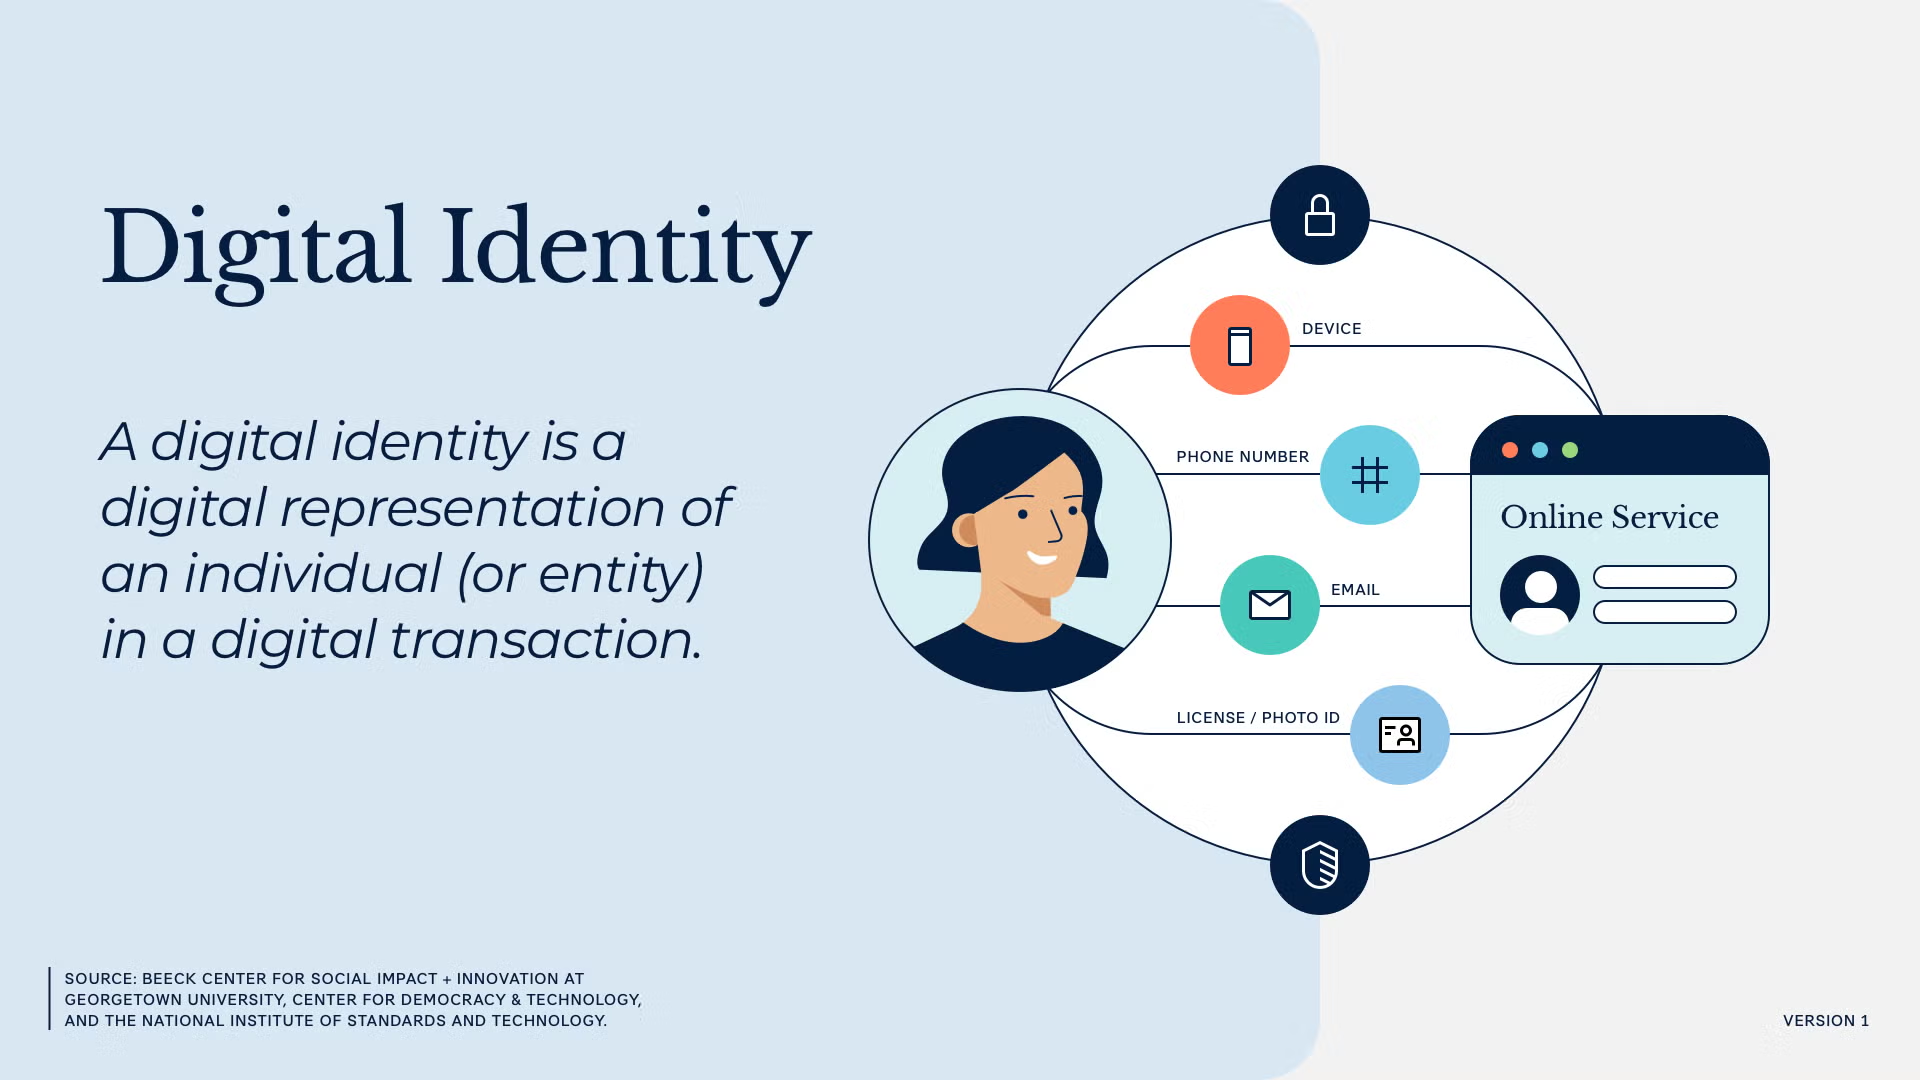
\includegraphics[width=\textwidth]{useridentity.png}
\end{frame}

\begin{frame}
	\frametitle{Identity Proofing}
	
	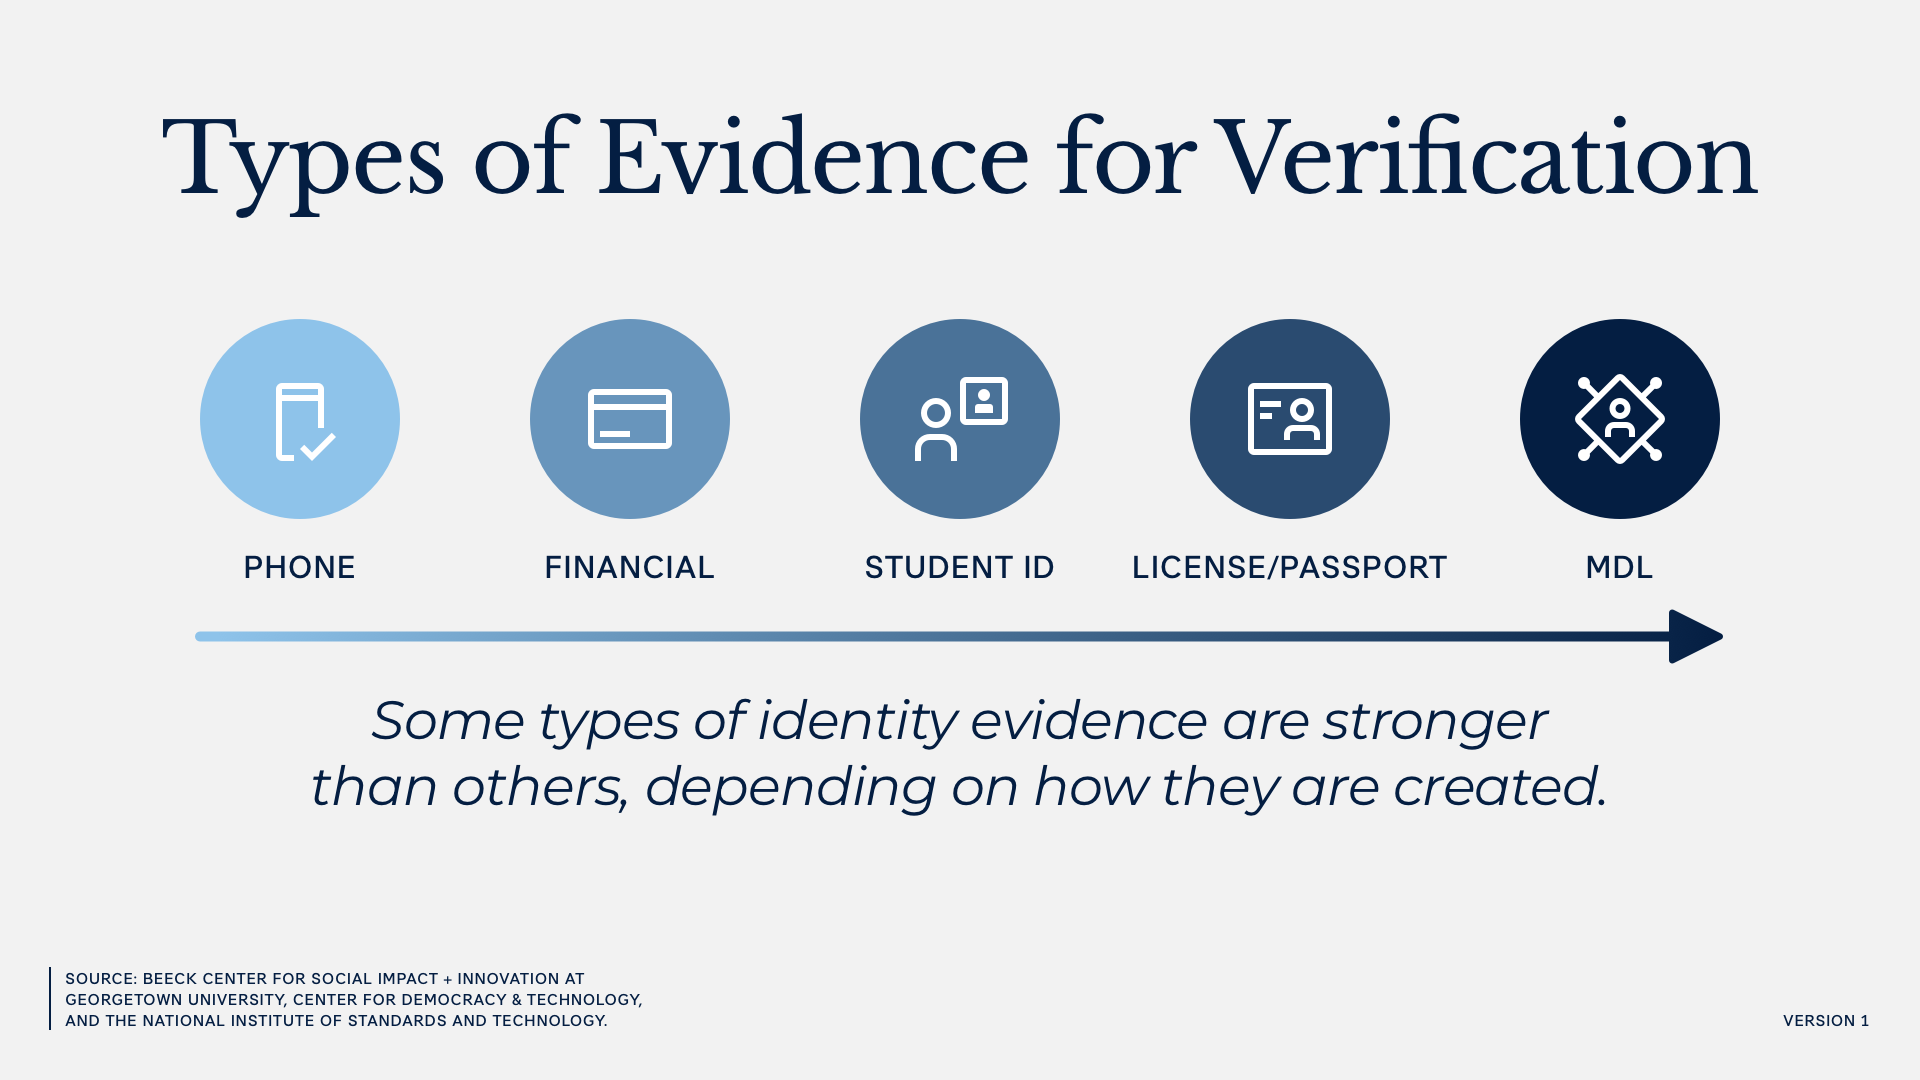
\includegraphics[width=\textwidth]{useridentityproofing.png}
\end{frame}

\begin{frame}
	\frametitle{Identity providers}
	
	\begin{itemize}
		\item In an enterprise a centralized database such as Active Directory acts as an identity provider, syncing with the master golden source such as HRMS.
		\item In a customer centric organization the CRM (Customer relationship management) serves as a golden source. Syncing from it the application sets up its authentication database using ORACLE or any such RDBMS
		\item Federated identity, Suppose the organization do not want its own identity provider they could integration with a third party provider such as Google or Microsoft. This arrangement is called as Federated identity.
	\end{itemize}
\end{frame}	
\begin{frame}
	\frametitle{Authentication}
	
	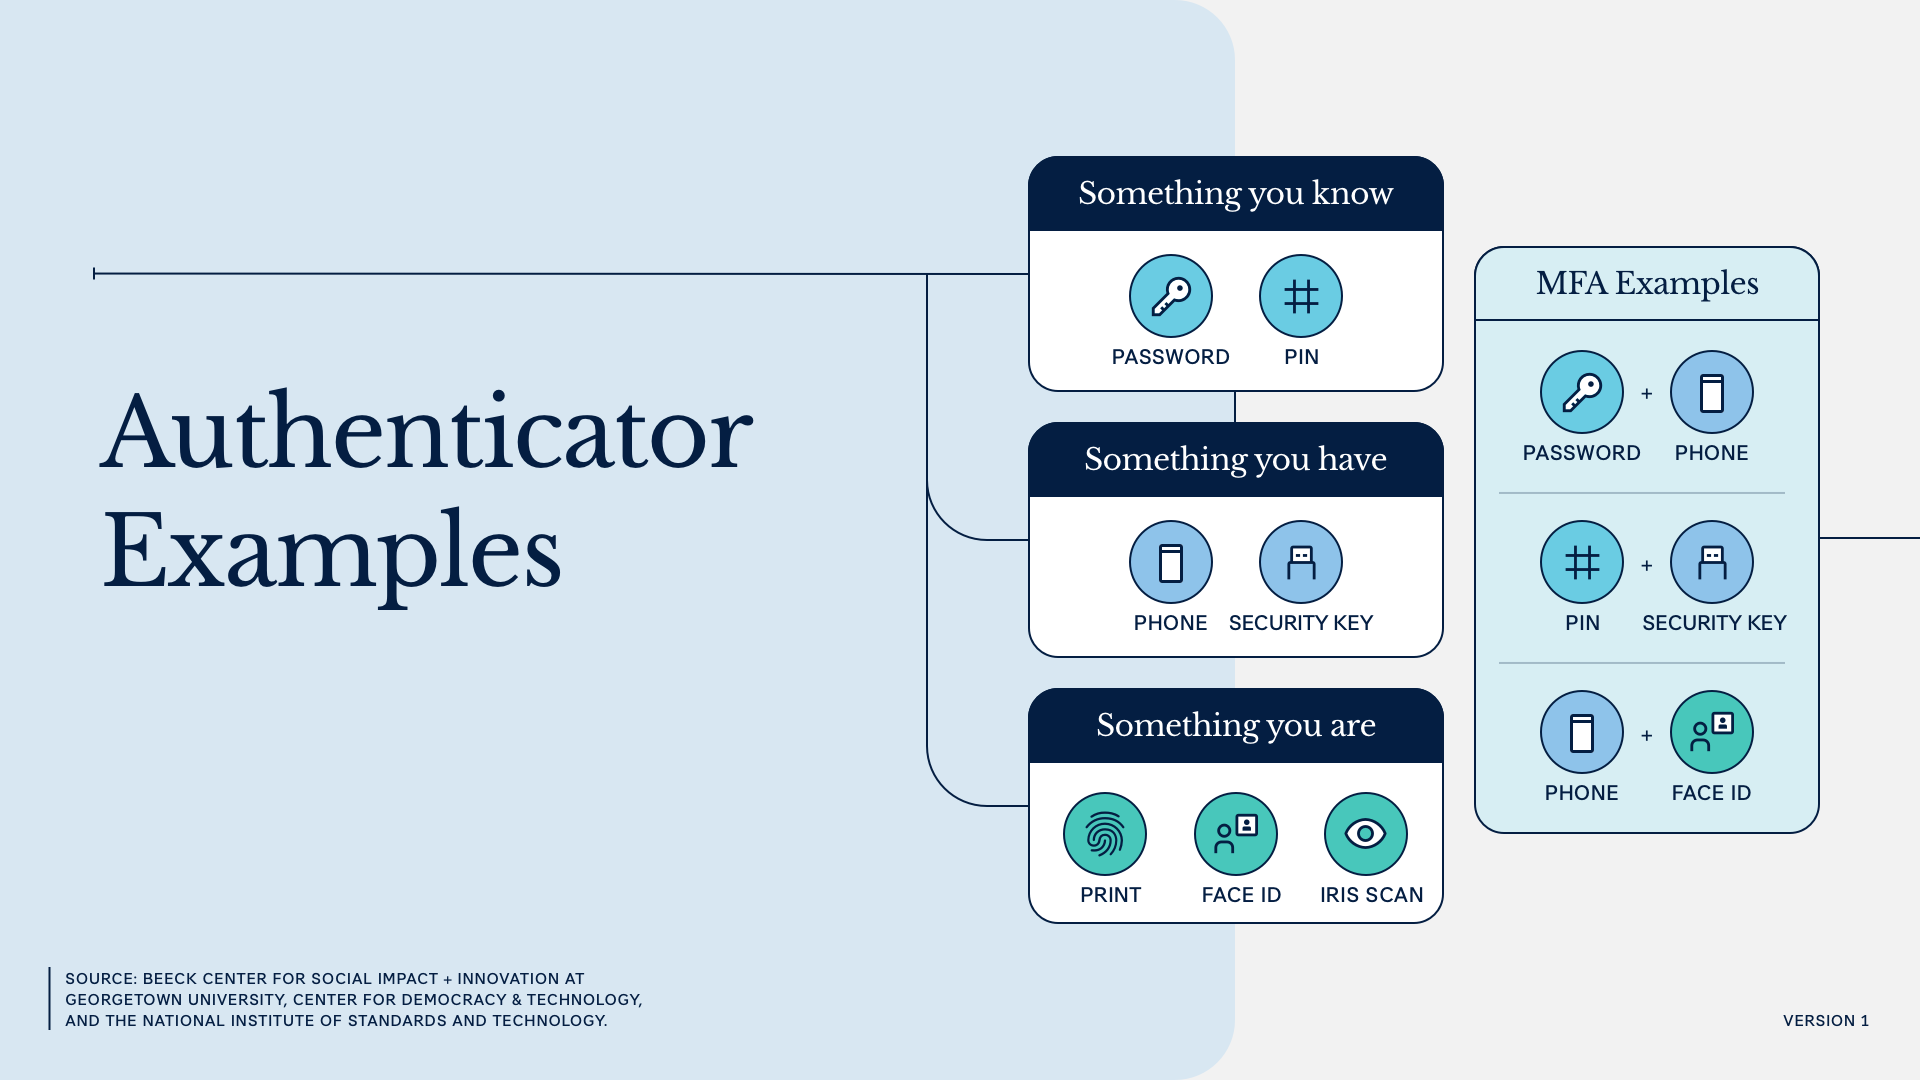
\includegraphics[width=\textwidth]{authentication.png}
\end{frame}	
	
\begin{frame}
	\frametitle{Identity and access management}
Identity and Access management (IAM) integrates all the definitions into one single workflow
\begin{itemize}
	\item Authentication is a building block to the larger concept Identity and Access management.
	\item The authentication workflow for every user involved validating the user identity and then determine within the application what functions / resources user can access.
	\item Additionally, IAM automates onboarding and offboarding of users, and also monitors their behavior inside your environment to spot any suspicious activity. 
\end{itemize}

NOTE: User provisioning, onboarding or de-provisioning and offboarding are terminologies used interchangeably.
\end{frame}	

\section{Implementating the envisaged operations in IAM}

\begin{frame}
	\frametitle{OIDC, OAUTH2.0 and JWT tokens}

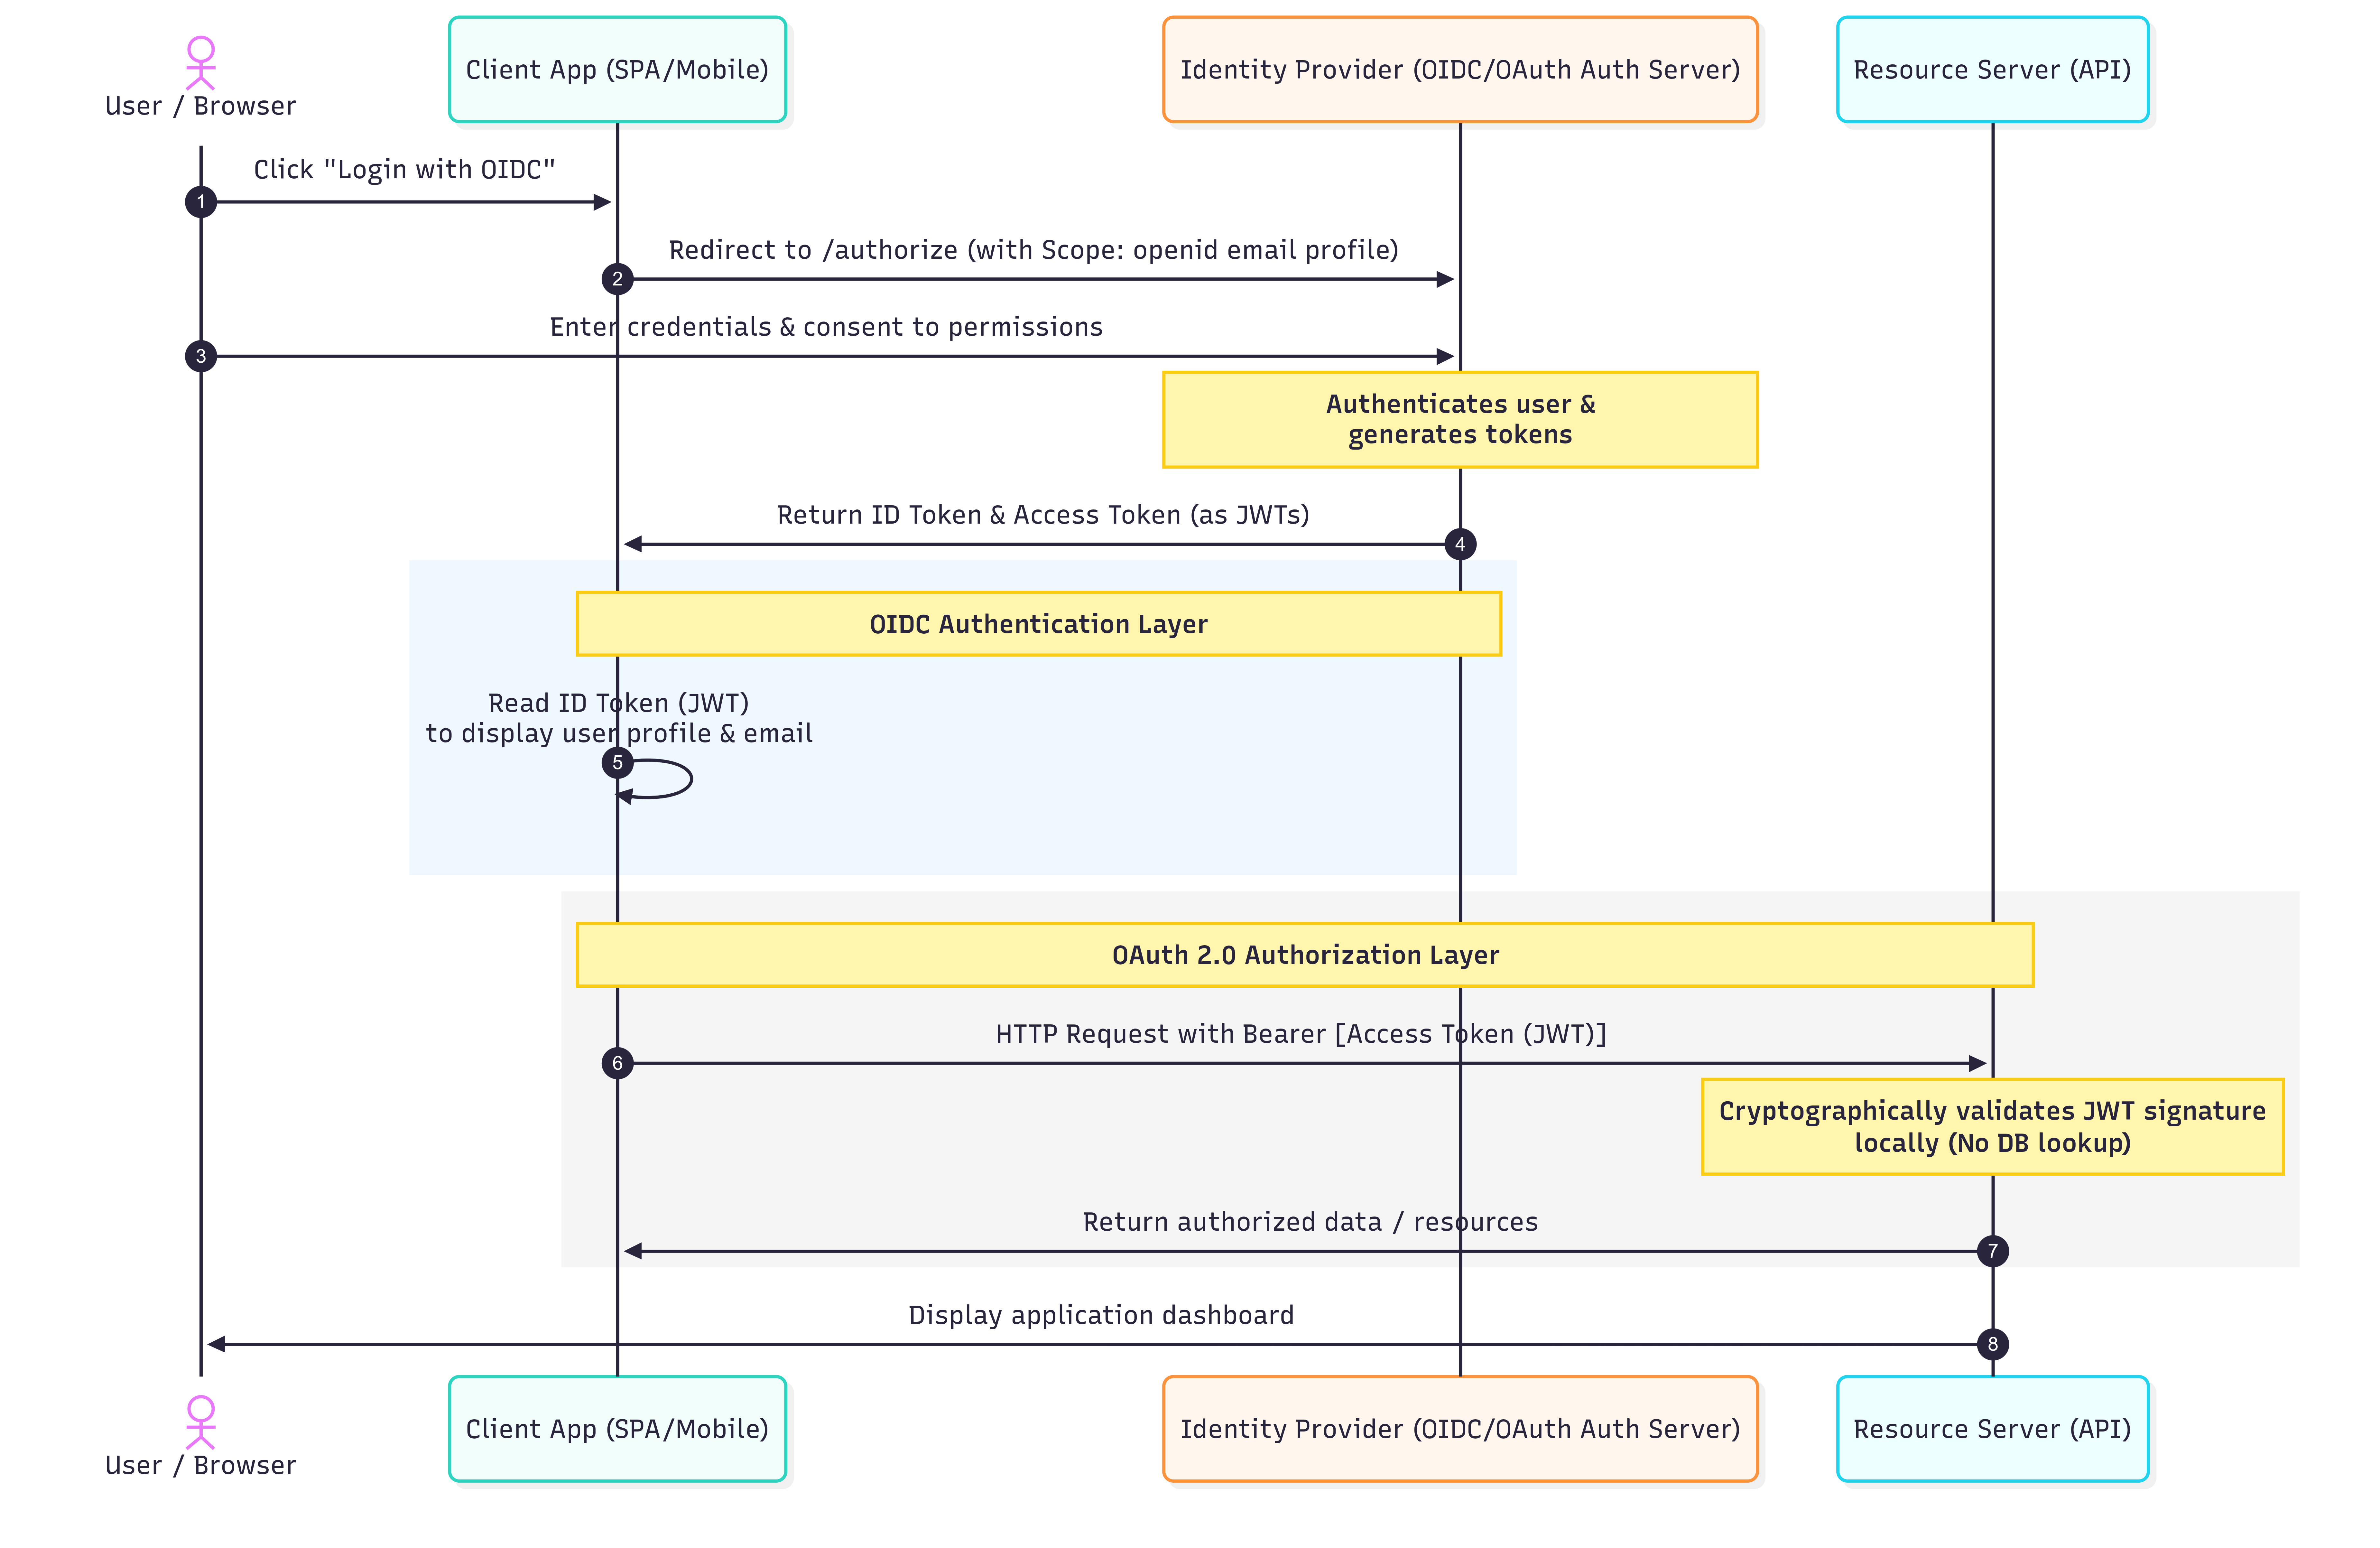
\includegraphics[width=.9\textwidth]{oidcflow.png}

\end{frame}	

\section{Literature}

\begin{frame}
	\frametitle{Notes}
\tiny	
	\begin{itemize}
		\item \url{https://heimdalsecurity.com/blog/what-is-user-provisioning/}
		\item \url{https://heimdalsecurity.com/blog/identity-and-access-management/}
		\item \url{https://digitalgovernmenthub.org/publications/digital-identity-101-an-introduction-to-digital-identity-in-public-benefits-programs/}
		\item \url{https://identitymanagementinstitute.org/identity-security-posture-management/}
		\item \url{https://www.codemag.com/Article/2312021/Web-Application-Authentication}
		\item \url{https://www.microsoft.com/en-in/security/business/security-101/what-is-openid-connect-oidc}
		\item \url{https://medium.com/@shubhamatucsd/the-complete-guide-to-oauth-2-0-openid-connect-and-jwt-token-verification-f2516c196f3b}
		\item \url{https://www.jwt.io/}
	\end{itemize}
	
\end{frame}

\begin{frame}
	\frametitle{Content references}

Common Golden Sources of IdentityOrganizations generally rely on one of three systems to serve as their primary source of truth:

\begin{itemize}
	\item HR Management Systems (HRMS): This is the most common golden source for internal employees. Examples include Workday, SAP SuccessFactors, or BambooHR. When HR hires an employee, the identity lifecycle automatically begins.
	\item Customer Relationship Management (CRM): This serves as the golden source for external identities, such as clients or citizens. Examples include Salesforce or HubSpot.
	\item Supplier/Vendor Portals: Used for third-party contractors and partners, ensuring their access is strictly tied to active procurement contracts.
\end{itemize}

\end{frame}

\begin{frame}
	\frametitle{Architectural checklists}
	
	\begin{itemize}
		\item What specific system (e.g., Workday, Active Directory, a custom SQL database) are you currently considering as your primary source?
		\item Are you managing internal employees, third-party contractors, or external customers?
		\item What Identity and Access Management (IAM) platform (e.g., Okta, Microsoft Entra ID, Ping Identity) are you planning to connect to this source?
	\end{itemize}
	
	
\end{frame}


\end{document}


